\subsection{Normalized Device Coordinates (NDC)}

In Normalized Device Coordinates, $x$, $y$ and $z$ $\in [-1,1]$. This is the default coordinate system in OpenGL. The following image shows the NDC space.

\begin{center}
    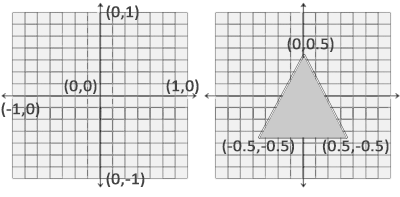
\includegraphics[scale = 3]{pics/ndc.png}
\end{center}

\subsection{Graphics Pipeline}

The order with which OpenGL proccesses vertex data:

\begin{center}
    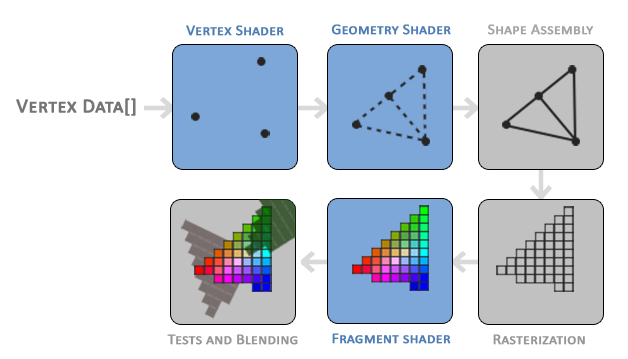
\includegraphics[scale = 2]{pics/pipeline.png}
\end{center}

\subsection{Vertex Buffer Data}

Vertex attributes are stored in the following order:

\begin{center}
    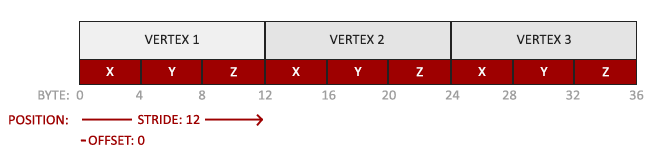
\includegraphics[scale = 0.5]{pics/vertex_attribute_pointer.png}
\end{center}

Vertices are stored in the Vertex Buffer Object (VBO).

We can also specify colors in the vertex buffer data. In the shader file, coordinates will be defined in \verb|location 0| and colors in \verb|location 1|.

\begin{center}
    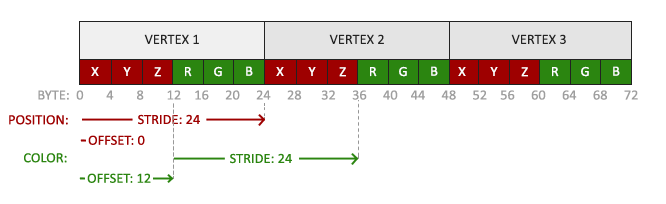
\includegraphics[scale = 0.5]{pics/vertex_attribute_pointer_interleaved.png}
\end{center}
\newpage
In the main file:

\begin{lstlisting}[language=C++]
    float vertices[] = {
        // positions         // colors
        0.5f, -0.5f, 0.0f,  1.0f, 0.0f, 0.0f,   // bottom right
        -0.5f, -0.5f, 0.0f,  0.0f, 1.0f, 0.0f,   // bottom left
        0.0f,  0.5f, 0.0f,  0.0f, 0.0f, 1.0f    // top 
    };   
\end{lstlisting}

In the shader file:

\begin{lstlisting}[language=C++]
    #version 330 core
    layout (location = 0) in vec3 aPos;   // the position variable has attribute position 0
    layout (location = 1) in vec3 aColor; // the color variable has attribute position 1
    
    out vec3 ourColor; // output a color to the fragment shader

    void main()
    {
        gl_Position = vec4(aPos, 1.0);
        ourColor = aColor; // set ourColor to the input color we got from the vertex data
    }       
\end{lstlisting}

\subsection{VBO, VAO, EBO}

\begin{itemize}
    \item \textbf{VBO} stores vertex data (e.g., positions, normals, colors) in GPU memory. \red{It allows efficient transfer of vertex data to the GPU, enabling faster rendering. You bind a VBO and then specify the vertex data using functions like glBufferData.}
    \item \textbf{VAO} stores the configuration of vertex attributes and their associated buffers. \red{It simplifies the process of switching between different vertex data configurations. When you bind a VAO, it automatically sets up the vertex attribute pointers and buffer bindings.}
    \item \textbf{EBO} stores indices that define the order in which vertices should be drawn. \red{It helps in reducing the amount of vertex data needed by reusing vertices. You bind an EBO and specify the indices using functions like glBufferData.}
\end{itemize}

\subsection{Shaders}

\subsection{Textures}

Texture coordinates in OpenGL are in range $[0,1] \times [0,1]$.

\begin{center}
    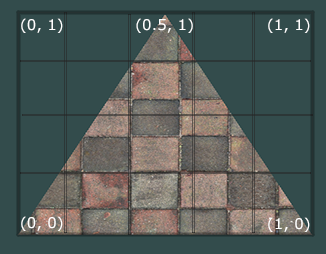
\includegraphics{pics/tex_coords.png}
\end{center}

Specifying coordinates outside this range, OpenGL will repeat the texture by default. There are also other options:

\begin{enumerate}
    \item \verb|GL_REPEAT|: Default.
    \item \verb|GL_MIRRORED_REPEAT|: Same as \verb|GL_REPEAT| but mirrors the image with each repeat.
    \item \verb|GL_CLAMP_TO_EDGE|: Clamps the coordinates between 0 and 1. The result is that higher coordinates become clamped to the edge, resulting in a stretched edge pattern.
    \item \verb|GL_CLAMP_TO_BORDER|: Coordinates outside the range are now given a user-specified border color.
\end{enumerate}

\begin{center}
    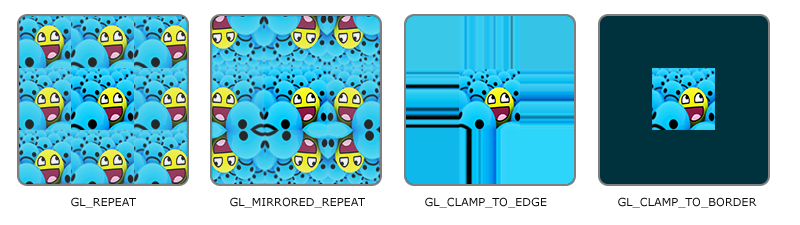
\includegraphics[scale=0.5]{pics/texture_wrapping.png}
\end{center}